\chapter{Introduction to normal mixture models}


%% it 3
\section{Definitions}

A good and thorough introductory book is the work of \cite{McL00} and
the reader is encouraged to study it to learn in depth about normal mixtures
and their clustering. 
We will here give a short overview of normal mixtures to fix notation and 
nomenclature.
The motivating idea behind mixture models is, that in real world examples
a sample might be suspected to arise from more than one population.
The example of this, that is generally considered to be the first of this kind,
is the one by Karl Pearson, who fitted two normal distributions with different 
means and variances.
In his book, \cite{Pea96}[Section 4.d.; page 266], Pearson analyzed measurements
of forehead to body length of crabs sampled from the bay of Naples. His mixture 
model-based approach suggested, that the crabs were evolving into two new 
subspecies.
%TODO: less confused desc of pearsons research

% it 2
While the theory of mixture models holds for a much broader class of 
distributions, we restrict ourselves here to the case of normal distributions,
because this restriction fits more comfortably into the scope of this work and 
because normal distributions allow for a convenient, parsimonious 
parametrization, that is of interest to study.

% it 1
normal gives easy param ov cov mats
multivariate builds on work done in the nor1mix package. 'filedrawer research'

Let $ \mu \in \mathbb{R}^p , \quad \Sigma \in \mathbb{R}^{p \times p} $ be
symmetric positive definite and $ \phi(- ; \mu, \Sigma) $ be the normal 
distribution with mean $ \mu $ and covariance matrix $ \Sigma $.


$ \pmb{Y}_1, \dots , \pmb{Y}_n $

\begin{definition}
    Suppose we have a random sample $ \pmb{Y}_1, \dots , \pmb{Y}_n $ with 
    probability density function $ \pmb{Y}_j \sim f(y_j) $ on 
    $\mathbb{R}^p$ We assume that the density $ f(y_j) $ of $ \pmb{Y}_j $ can 
    be written in the form 
    \[ f(y_j) = \sum_{k=1}^{K} \pi_k \phi_k (y_k; \mu, \Sigma) \]
    The $ \pi_k $ are called the component densities of the mixture and the 
    $\phi_k$ mixture components.
\end{definition}

% it 1
For 'large' datasets there are more parsimonious parametrizations, that reduce
computation time. These, for example, assume that all components have the same
covariance, or have certain restrictions placed on them. We will give a 
detailed description of the models assumed in this thesis in section 
\ref{sec:models}.


\section{The EM-Algorithm in Sketch}

%% it 1
With this definition we immediately face the problem of how to fit these
mixture components to given data. A popular algorithm to solve this problem 
is the {\bf E}xpectation-{\bf M}aximization algorithm, abbreviated as 
EM-algorithm.

We give here a sketch of the EM-algorithm in the case of all normal mixture 
components, since it is the scope of this thesis and simplifies it 
considerably. %TODO: rewrite this sentence

Suppose we have a $p-$dimensional dataset of $n$ samples $x_1, \dots ,x_n$,
onto which we would like to fit $K$ normal distributions 
$\phi_k,\ k \in {1,\dots , n}$. 
We introduce a further explaining variable $\pmb{Z}$ in 
$\textrm{Mat}^{n\times k}$, with entries in $[0,1]$ which represent the 
expectation that observation $i$ belongs to component $k$.

The EM-algorithm is a two step, iterative process consisting of an 'e'-step
and an 'm'-step.
% FIXME: inconsistent notation in Z and \tau
% FIXME: add remark about
In the e-step the expectation of component membership is updated.
\[ \tau_i(y_j;\Psi) = \phi_i(y_j;\mu_i, \Sigma_i)/ \sum_{k=1}^K \phi_k(y_j;
    \mu_k, \Sigma_k)\]
and in the m-step given the component membership information we update the 
component means and covariances by weighted versions of the usual estimators.
\[\mu_i = \sum_{j=1}^n \tau_{ij}y_j / \sum_{j=1}^n \tau_{ij}\]
\[\Sigma_i = \sum_{j=1}^n \tau_{ij} (y_j- \mu_i)(y_j-\mu_i)^\top / 
    \sum_{j=1}^n \tau_{ij}\]

here note about initialization methods.

% it 1
While it is possible to use a purely EM-based approach, most popular 
implementations use some form of pre clustering and use the EM-algorithm as
final pass to fit the data. The R-package {\tt Mclust} for example uses 
hierarchical agglomerative clustering \cite{Scr16}.



\section{Choice of Notation}

% it 1
The classification of models in this paper relies heavily on the work of 
\cite{Cel95}, however, out of necessity for clarity, we break with their 
notation. 
So as to not confuse the reader we describe here in depth the differences in 
notation between \cite{Cel95} and ours.

The basis of classification in \cite{Cel95} is the decomposition of a
symmetric matrix into an orthogonal and a diagonal component.
A symmetric positive definite matrix $ \Sigma $ can be decomposed as follows
    \[ \Sigma = \lambda \pmb{D} \pmb{A} \pmb{D}^{\top} \]
with $ \pmb{D} $ an orthogonal matrix and $ \pmb{A} $ a diagonal matrix and
$ \lambda = \sqrt[\uproot{3}p]{det(\Sigma)} $ the $ p-th $ root of the 
determinant of $ \Sigma $.

This decomposition has an appealing geometric interpretation, with $ \pmb{D} $ 
as the \textit{orientation} of the distribution, $ \pmb{A} $ the \textit{shape},
and $ \lambda $ the \textit{volume}. The problem of notation comes from standard 
conventions in linear algebra, where the letters $A$ and $D$ are usually 
occupied by arbitrary and diagonal matrices respectively. Furthermore, we intend
to apply a variant of the Cholesky decomposition to $ \Sigma $, the 
$ \alpha\pmb{L}\pmb{D}\pmb{L}^{\top} $ decomposition. This obviously raises some
conflicts in notation.

Therefore we, from here on, when referring to the decomposition as described by 
\cite{Cel95}, will use the following modification of notation:

\begin{gather*} 
    \pmb{D} \longmapsto \pmb{Q} \\
    \pmb{A} \longmapsto \pmb{\Lambda} \\
    \lambda \longmapsto \alpha  \\
    \Sigma = \lambda \pmb{D} \pmb{A} \pmb{D}^\top =
        \alpha \pmb{Q} \pmb{\Lambda} \pmb{Q}^\top
\end{gather*}

These were chosen according to general conventions of linear algebra. $ \pmb{Q} $
is usually chosen for orthonormal matrices; $ \pmb{\Lambda} $ is often a choice 
for diagonal matrices eigenvectors and $ \alpha $ was somewhat arbitrarily 
chosen.


\section{Models of Covariance Matrices}
\label{sec:models}

make clear that the models can not be translated one to one to ldlt model
% it 1
There is however an issue with the Cholesky decomposition. For 10 out of 14
cases as defined by \cite{Cel95}, there exists a canonical translation of
decompositions.
The 6 diagonal cases need no translation; the eigen and Cholesky decomposition
are equal to identity.
For the non-diagonal cases note that for a given sym. pos. def. matrix
$ \Sigma $ we have decompositions:
\[\Sigma = \alpha \pmb{Q \Lambda Q}^\top \quad \Sigma =\alpha \pmb{L D L}^\top\]
Since in both cases the bracketing matrices $ \pmb{Q} $ and $ \pmb{L} $ have 
determinant $ 1 $ the determinant of $ \Sigma $ falls entirely on $ \alpha $.
Therefore $ \alpha $, in these particular decompositions, is equal for both.
Celeux \& Grovaert vary $\Sigma$ by either varying or holding fixed the volume 
$(\alpha / \alpha_k)$, shape $(\pmb{\Lambda} / \pmb{\Lambda_k})$ and orientation
$(\pmb{Q} / \pmb{Q}_k)$.
These 3 times 2 cases would yield the 8 out of 14 cases of non-diagonal cases.
However there is no canonical transform for either variable orientation and 
fixed shape or fixed orientation and variable shape.
The reason for this is that in the $\pmb{LDL}^\top$ decomposition the lower
diagonal matrix $\pmb{L}$ holds some of the shape of the matrix, which in 
the eigendecomposition is in the $\pmb{\Lambda}$ matrix.
In fact, $\pmb{L}$ is orthogonal if and only if 
$\pmb{L} = \mathrm{Id}_{n\times n}$.
Therefore we can only decompose matrices where either both or neither shape and
orientation vary. See table \ref{table:param}.

While we could in theory construct the cases $\pmb{L}\pmb{D}_k\pmb{L}^\top$ and
$\pmb{L}_k \pmb{D} \pmb{L}^\top$, however they do not correspond to the desired
geometric intent behind the differentiation of models and are therefore not 
included.


\begin{table}[!htb]
    \centering
\rotatebox{90}
{
    \begin{tabular}{| c | c c c c c | c c c |}
        \hline
        Model & $\pmb{\Sigma}_k$ C\&G & volume & shape & orientation & parameters & $ \pmb{LDL}^\top $ & parameters & count \\
        \hline

        EII    & $ \alpha \pmb{I} $ & equal & equal & - & $ \alpha $ & as in C\&G & & 1 \\
        VII    & $ \alpha_k \pmb{I} $         & var. & equal & - & $ \alpha_k $ & & & $K$  \\
        EEI    & $ \alpha \pmb{\Lambda} $     & equal & equal & coord. axes & $ \alpha, \lambda_i $ & & & $ 1+(p-1) $\\
        VEI    & $ \alpha_k \pmb{\Lambda} $ & var. & equal & coord. axes & $ \alpha_k, \lambda_{i}$ & & & $ K+(p-1) $ \\
        EVI    & $ \alpha \pmb{\Lambda}_k $ &equal & var. & coord. axes & $ \alpha, \lambda_{i,k} $ & & & $ 1+K(p-1) $ \\
        VVI    & $ \alpha_k \pmb{\Lambda}_k $ & var. & var. & coord. axes & $ \alpha_k, \lambda_{i,k} $ & & & $ K+K(p-1) $ \\
        \hline
        EEE    & $ \alpha \pmb{Q \Lambda Q}^\top $ &equal & equal & equal & $ \alpha, \lambda_{i}, q_{i,j} $ & $ \alpha \pmb{LDL}^{\top} $ & $ \lambda , d_i, l_{i,j} $ & $ 1+(p-1)+\frac{p(p-1)}{2} $ \\
        \hline
        EVE    & $ \alpha \pmb{Q \Lambda}_k \pmb{Q}^\top $ &equal & var. & equal & $ \alpha, \lambda_{i,k}, q_{i,j} $  & doesn't exist & & $ 1+K(p-1)+\frac{p(p-1)}{2} $ \\
        \hline
        VEE    & $ \alpha_k \pmb{Q \Lambda Q}^\top $ & var. & equal & equal & $ \alpha_k, \lambda_{i}, q_{i,j} $ & $ \alpha_k \pmb{LDL}^\top $ & $ \lambda_k , d_i, l_{i,j} $ & $ K+p+\frac{p(p-1)}{2} $ \\
        \hline
        VVE    & $ \alpha_k \pmb{Q \Lambda}_k \pmb{Q}^\top $ &var. & var. & equal & $ \alpha_k, \lambda_{i,k}, q_{i,j} $ & & & $ K+K(p-1)+\frac{p(p-1)}{2} $ \\
        EEV    & $ \alpha \pmb{Q}_k \pmb{\Lambda} \pmb{Q}_k^\top $ &equal & equal & var. & $ \alpha, \lambda_{i}, q_{i,j,k} $ &  don't exist  & & $ 1+(p-1)+K\frac{p(p-1)}{2} $ \\
        VEV    & $ \alpha_k \pmb{Q}_k \pmb{\Lambda} \pmb{Q}_k^\top $ &var. & equal & var. & $ \alpha_k, \lambda_{i}, q_{i,j,k} $ & & & $ K+(p-1)+K\frac{p(p-1)}{2} $ \\
        \hline
        EVV    & $ \alpha \pmb{Q}_k \pmb{\Lambda}_k \pmb{Q}_k^\top $ & equal & var. & var. & $ \alpha, \lambda_{i}, q_{i,j,k} $ & $ \alpha \pmb{L}_k \pmb{D}_k \pmb{L}_k^\top $ & $ \lambda, d_{i,k}, l_{i,j,k}\ j>i $ & $ 1+pK+K\frac{p(p-1)}{2} $  \\
        VVV    & $ \alpha_k \pmb{Q}_k \pmb{\Lambda}_k \pmb{Q}_k^\top $ & var. & var. & var. & $ \alpha_k, \lambda_{i}, q_{i,j,k} $ & $ \alpha_k \pmb{L}_k \pmb{D}_k \pmb{L}_k^\top $ & $ \lambda_k, d_{i,k}, l_{i,j,k}\ j>i $ & $ K+pK+K\frac{p(p-1)}{2} $ \\
        \hline
    \end{tabular}
}

\caption{Table of Parameters}
\label{table:param}
\end{table}

\clearpage


\section{Problems of EM}


The EM-algorithm has stalling problems especially close to a local optimum.
% it 1
In their seminal work, \cite{Dem77}, have proven that the EM-algorithm 
converges under mild regularity conditions. 
%TODO: talk more about Dem77, in more detail about convergence conditions
However, convergence does not guarantee fast convergence. In fact, a lot of 
the work, that has gone into the research around the EM-algorithm has been 
concerned with speeding up convergence, see \cite{McL00}[section 2.17].
In common software implementations, %TODO: mostly initial clustering?? not sure
The concern here is that a slowing in convergence might be mistaken for actual
convergence.

% it 1
This phenomenon is not infrequent and in difficult mixtures quite visible.
To illustrate let us look at a particular mixture taken from \cite{Mar92} and
the {\tt nor1mix} package from CRAN.



\begin{figure}[h]
    \centering
    \begin{minipage}{0.45\textwidth}
\begin{Schunk}
\begin{Sinput}
>     library("nor1mix")
>     MW.nm9 ## Trimodal mixture
\end{Sinput}
\begin{Soutput}
'Normal Mixture' object 	 ``#9 Trimodal'' 
       mu sigma    w
[1,] -1.2  0.60 0.45
[2,]  1.2  0.60 0.45
[3,]  0.0  0.25 0.10
\end{Soutput}
\end{Schunk}
        \caption{Parameters of {\tt MW.nm9}}
        \label{tab:MW.nm9}
    \end{minipage}
    \begin{minipage}{0.45\textwidth}
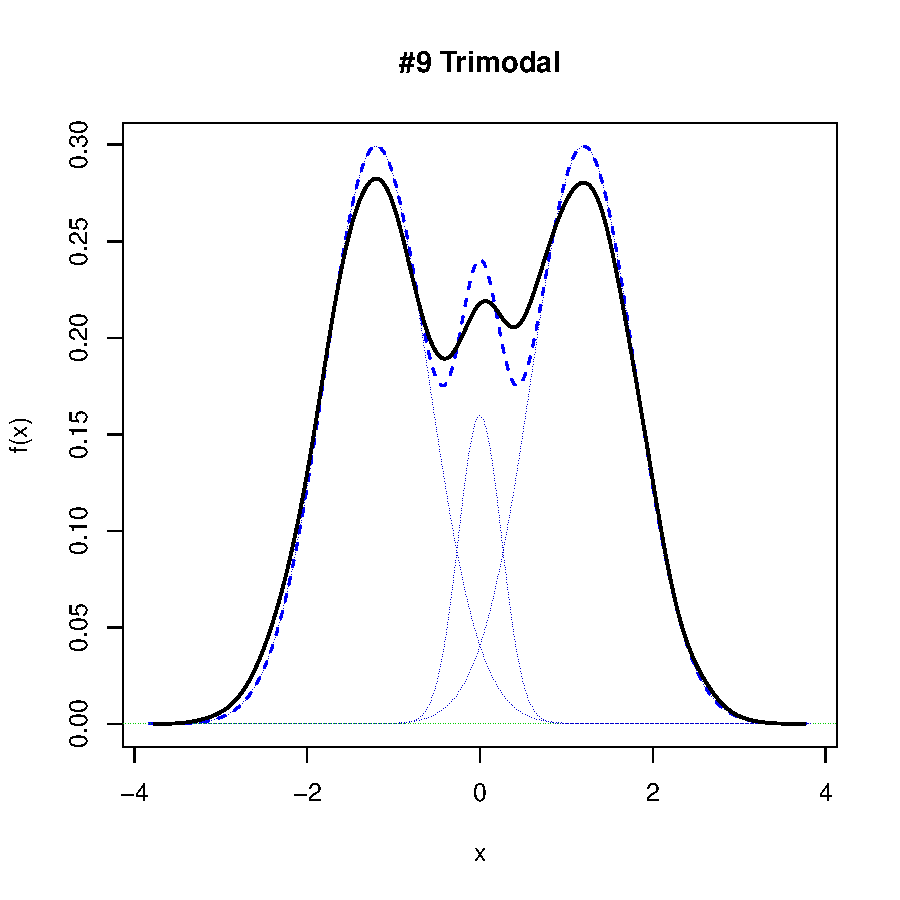
\includegraphics{chapter1-figTrimodal}
        \caption{True and Estimated density}
        \label{fig:MW.nm9}
    \end{minipage}
\end{figure}
% TODO: fix placement issue and caption location

then an illustration of MW examples of pathological cases



%yay, got figure to print. solution was use of fig=TRUE, instead of various mutations like figure=true.

here we see how change in loglik seems to stagnate. However, this does not stay that way, if we let EM run a bit further.


\begin{figure}[h]
    \centering
    \begin{minipage}{0.45\textwidth}
    \centering
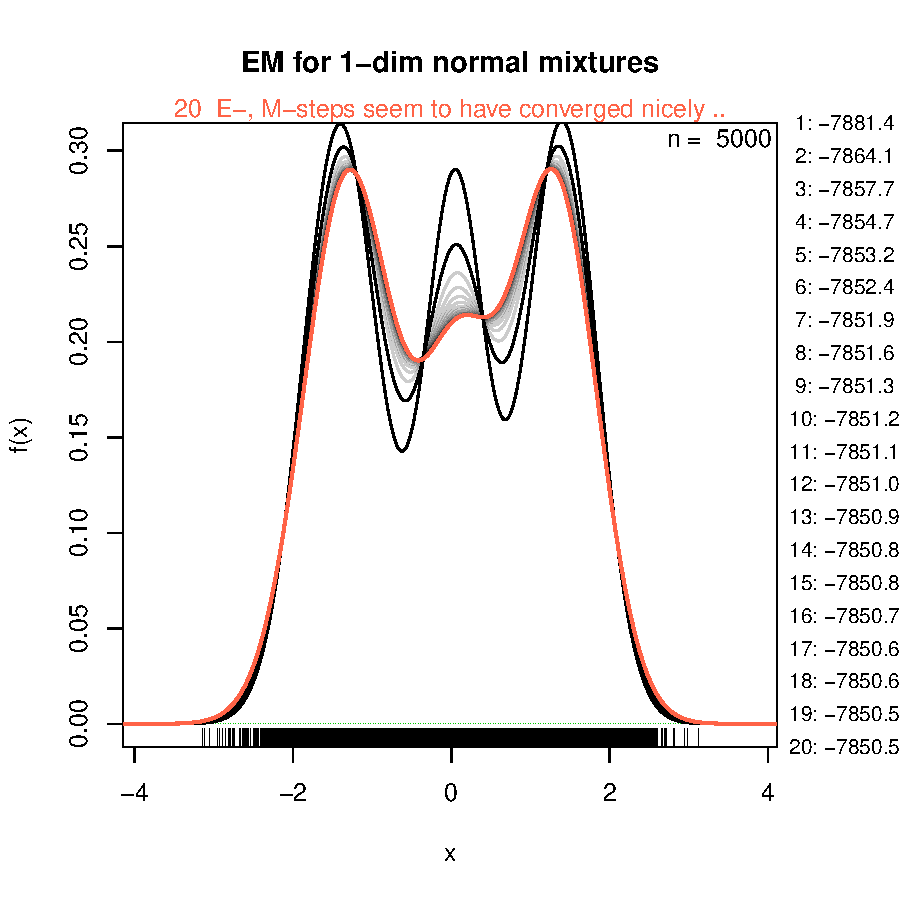
\includegraphics{chapter1-fignor1mixEx}
    \caption{20 EM steps}
    \end{minipage}\hfill
    \begin{minipage}{0.45\textwidth}
    \centering
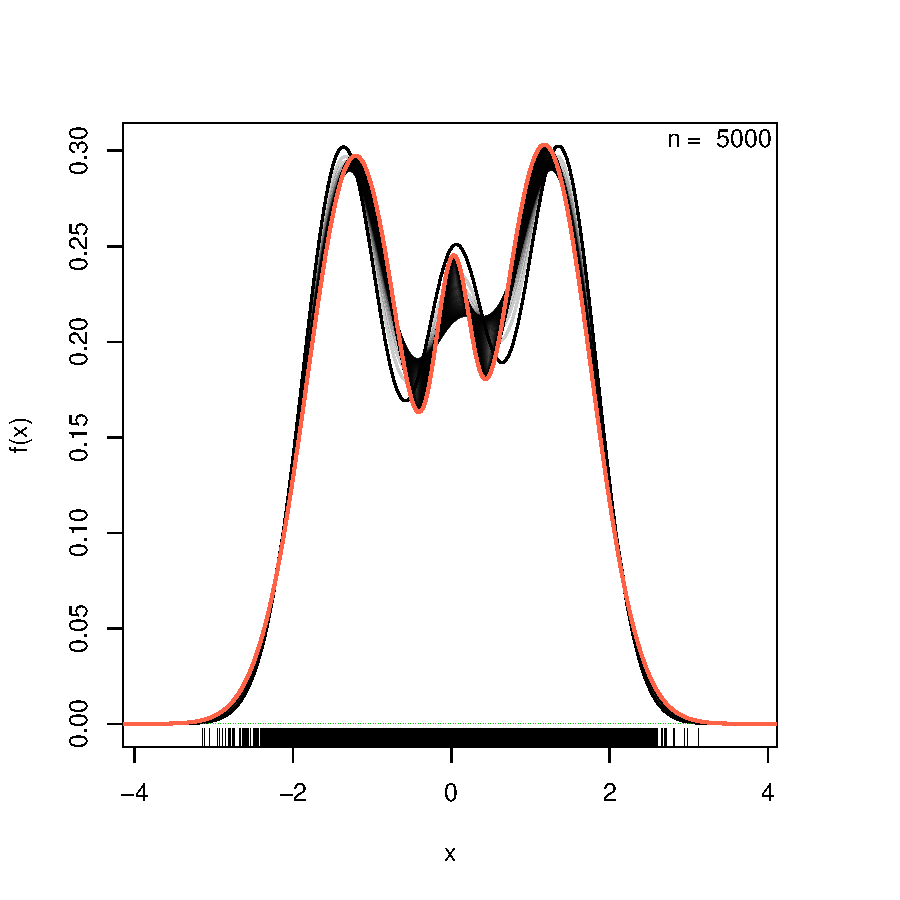
\includegraphics{chapter1-figplotemsteps}
    \caption{200 EM steps}
    \end{minipage}
    \label{adfafdafds}
\end{figure}

to conclude example show part of mixest that shows it takes 1200 iterations to converge

In fact, it seems that the previous solution is a saddle point in the likelihood function, where EM has chronic problems continuing improvements.

give 2D demonstration.

maybe show Marr Wand's examples of 'difficult' mixtures

give conclusion recapping the just demonstrated, and lead in for next chapter

